\section{External validation on Celebrity}\label{sec:external}
\subsection{Target audit and evaluation protocol}
We evaluate transfer to Celebrity, a separate web-collected fake/legitimate news collection from P\'erez-Rosas et al.~\cite{perezrosas2018automatic}. The supplied version contains 500 articles, 250 per label; it is distinct from the crowdsourced FakeNewsAMT collection in the same archive, which we do not use. The original authors describe manual checking against gossip-verification sites and other reporting. We retain their labels rather than independently adjudicating every article. Celebrity is used only as an external target, not a fourth training corpus, and its size falls below our original 3,000-per-class training-corpus threshold.

The audit compares all 500 items with every row of the frozen 61,197-document source analysis input, using normalized exact, prefix and primary/sensitivity near-duplicate checks. It records nine evidence rows involving two Celebrity articles: \texttt{062legit.txt} overlaps ISOT-12805 and \texttt{062fake.txt} overlaps WELFake-58856. Manual inspection records shared content; the ISOT/Celebrity label conflict is unresolved. A separate item, \texttt{131fake.txt}, has only one 28-word physical line and no body under our first-line-as-headline rule. We exclude provisional numeric groups 062 and 131 conservatively, retaining \textbf{496 articles, 248 per label}. Numeric groups remain provisional story links, not verified semantic pairs. No internal near-duplicate candidates meet the tested thresholds. These screens reduce detected overlap without establishing complete independence. Long articles and fact-checking/publisher-language flags are retained; a legitimate interview explicitly dates itself to 1974, so this is not a temporal holdout.

The external protocol was fixed before external scoring, after the three-corpus results were known, without formal registration. Models are retrained only on the original source corpora, retaining their configurations, seeds 0--7 and paired source selections. Every model covers C0, E, $R_E$, S+E, $R_{SE}$, L, L+E, L+$R_E$, S+L+E and L+$R_{SE}$: \textbf{240 fits per model, 720 total}. The additional S+E/$R_{SE}$ transformer pair belongs to this extension; it does not fill an omitted cell of the earlier validation. No target score is used to select hyperparameters, masking rules or checkpoints. The initial operational pilot is one job of this same frozen grid and is retained.

Primary comparisons are E minus $R_E$ and S+E minus $R_{SE}$ on all 496 eligible articles. Target IDs are fixed across seeds, source corpora and models, and random deletion matches the number of whole words removed from each document. Secondary L+E minus L+$R_E$ and S+L+E minus L+$R_{SE}$ comparisons use a separate, frozen \textbf{428-article target, 214 per label}, constructed by class-balanced length-bin sampling. These diagnostics use target labels and must not be compared with primary scores as if the target articles were identical. We report each source transfer separately, with means, sample standard deviations (SD), ranges and seed values; we introduce no external source pooling or new significance-test family. Seed variation conditions on the fixed target, not independent target samples.

\subsection{Source-specific results}
All 720 fits completed. Original source selections match all 24 saved model/seed manifests from the three-corpus study. Recorded pairing, target labels/IDs, deletion budgets, code hashes and result checksums pass verification. Independent aggregation reproduces all 288 seed/source/model AUC differences and 90 source-condition AUC summaries. These checks do not repeat training or independently recalculate metrics from per-article predictions, which were not exported. Online Resource 2 provides the saved outputs and CPU rebuild; Appendix~\ref{sec:external_appendix} gives baseline and secondary results and per-seed contrasts.

\begin{table}[t]
\caption{Celebrity primary comparisons on the fixed 496-article target: mean cross-dataset AUC difference (sample SD) across eight training seeds. Positive favors masking over matched random deletion. SD describes seed variation, not article-sampling uncertainty. Residual: constructed WELFake residual.}\label{tab:celebrity_primary}
\centering\footnotesize
\adjustbox{max width=\linewidth}{\begin{tabular}{@{}llccc@{}}
\toprule
Source & Contrast & TF-IDF & DistilBERT & RoBERTa\\
\midrule
ISOT & E $-$ $R_E$ & +0.0045 (0.0062) & -0.0176 (0.0324) & -0.0342 (0.0559)\\
ISOT & S+E $-$ $R_{SE}$ & +0.0025 (0.0044) & +0.0159 (0.0400) & -0.0033 (0.0421)\\
McIntire & E $-$ $R_E$ & +0.0095 (0.0024) & +0.0035 (0.0117) & -0.0200 (0.0176)\\
McIntire & S+E $-$ $R_{SE}$ & +0.0092 (0.0074) & +0.0205 (0.0159) & +0.0044 (0.0226)\\
Residual & E $-$ $R_E$ & +0.0164 (0.0057) & +0.0081 (0.0353) & +0.0501 (0.0283)\\
Residual & S+E $-$ $R_{SE}$ & +0.0176 (0.0086) & +0.0409 (0.0390) & +0.0665 (0.0265)\\
\bottomrule
\end{tabular}
}
\end{table}

TF-IDF's E-minus-$R_E$ means are positive from all sources (Table~\ref{tab:celebrity_primary}; Fig.~\ref{fig:celebrity_entity}). McIntire and residual means are $+0.0095$ and $+0.0164$, positive in eight of eight seeds; ISOT is smaller ($+0.0045$), positive in six of eight. This is qualified external support for the lexical-model pattern, rather than an identical effect magnitude. DistilBERT's corresponding means are $-0.0176$, $+0.0035$ and $+0.0081$ from ISOT, McIntire and the residual, with mixed signs across seeds. Its negative three-corpus pooled entity result does not transfer uniformly to Celebrity.

\begin{figure}[t]
\centering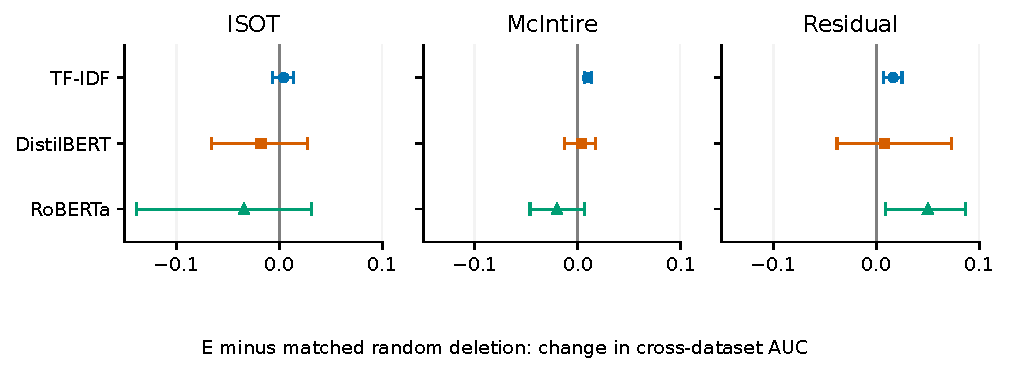
\includegraphics[width=\linewidth]{fig_celebrity_entity.pdf}
\caption{Celebrity primary E minus $R_E$ by training source. Points are means and whiskers are the observed minimum and maximum across eight seeds, \emph{not confidence intervals}. All fits use the same 496 target articles.}\label{fig:celebrity_entity}
\end{figure}

RoBERTa's primary entity means are $-0.0342$ from ISOT, $-0.0200$ from McIntire and $+0.0501$ from the residual; only the residual contrast is positive in every seed. Its primary S+E-minus-$R_{SE}$ mean from the residual is also positive in every seed ($+0.0665$). Source dependence is particularly clear in the secondary combined comparison: RoBERTa's S+L+E-minus-L+$R_{SE}$ difference is negative in all seeds from ISOT ($-0.0332$) and positive in all seeds from the residual ($+0.0866$); the McIntire mean is near zero ($+0.0011$). DistilBERT's residual-trained secondary combined contrast is positive in all seeds ($+0.0540$). These directions describe this fixed target and protocol; sign consistency alone is not a new significance claim.

Raw improvements and matched-control contrasts can point to different interpretations. For McIntire-trained RoBERTa, C0 scores 0.6521, E scores 0.7365, and $R_E$ scores 0.7566: the raw E gain is $+0.0845$, but E minus $R_E$ is $-0.0200$. Conversely, McIntire-trained TF-IDF scores 0.5835 under C0 and 0.5837 under E, despite an E-minus-$R_E$ difference of $+0.0095$. Beating random deletion need not mean beating C0. We therefore retain the original three-corpus gap estimates separately and interpret the external evidence through matched comparisons and source-specific reporting.
